% IEEE CONFERENCE TEMPLATE FOR EMOTION DETECTION PAPER
\documentclass[conference]{IEEEtran}

\usepackage[utf8]{inputenc}
\usepackage{amsmath,amssymb,amsfonts}
\usepackage{graphicx}
\usepackage{textcomp}
\usepackage{xcolor}
\usepackage{booktabs}
\usepackage[hidelinks]{hyperref}

\def\BibTeX{{\rm B\kern-.05em{\sc i\kern-.025em b}\kern-.08em
    T\kern-.1667em\lower.7ex\hbox{E}\kern-.125emX}}

\begin{document}

\title{Bidirectional LSTM with Attention for\\
Text-Based Emotion Classification}

\author{\IEEEauthorblockN{Anisha Kumari$^{1}$ and Avoy Nath Chowdhury$^{2}$}
\IEEEauthorblockA{$^{1}$Department of Computer Science and Engineering, \\
Motilal Nehru National Institute of Technology (MNNIT), Allahabad, Uttar Pradesh, India}
\IEEEauthorblockA{$^{2}$Department of Computer Science and Engineering, \\
Kalinga Institute of Industrial Technology (KIIT), Bhubaneswar, Odisha, India}
\IEEEauthorblockA{anisha.mishra@mnnit.ac.in, avoynath2004@gmail.com}}

\maketitle

\begin{abstract}
Emotion detection from text is a critical capability for understanding human sentiment in digital communication, with applications spanning mental health monitoring, customer service, and human-computer interaction. Traditional models often fail to capture bidirectional context and provide limited interpretability, while class imbalance in real-world datasets degrades minority emotion recognition. This paper presents a BiLSTM-Attention architecture for six-class emotion classification, using frozen 100-dimensional GloVe embeddings, a bidirectional LSTM encoder (128 units per direction), Bahdanau-style additive attention (128 units), and a compact dense head (64 units). The model is evaluated on the DAIR-AI dataset using a deterministic pipeline with fixed seeds and reports 93.2\% accuracy, 90.63\% Macro F1, and 93.33\% Weighted F1 on a 4,000-sample held-out test set. The final architecture contains approximately 1.81 million parameters, of which about 1.53 million belong to the frozen embedding layer, providing a reproducible and interpretable baseline for resource-constrained emotion classification systems.

\end{abstract}

\begin{IEEEkeywords}
Emotion Detection, BiLSTM, Attention Mechanism, Natural Language Processing, Deep Learning
\end{IEEEkeywords}

\section{Introduction}
Emotion detection from text is an emerging analytical capability in natural 
language processing paradigms which aims to identify specific emotional 
states such as joy, sadness, anger, fear, love, and surprise. Developers 
and researchers can build context-aware applications without having to 
rely on manual feature engineering. A number of challenges and issues are 
associated with the performance of text-based emotion classification 
environments. One of the most significant issue is the failure to capture 
long-range sequential dependencies, which resultant from the use of 
traditional shallow models relying heavily on bag-of-words and TF-IDF 
representations. In natural language communication, the linguistic 
executions are contextual in nature i.e, emotion is expressed through 
sarcasm, irony, and context-dependent phrasing. Once an utterance is 
processed without its sequence, any contextual cues that were present 
will be lost. When a short, informal, and noisy social media text is 
evaluated, standard grammatical rules are routinely violated which takes 
away crucial meaning before the actual classification starts. The impact 
of this limitation is referred to as the lack of contextual understanding. 
In accuracy sensitive applications, such as real-time mental health monitoring 
on the Internet of Things (IoT) or dynamic customer service routing, which 
requires immediate attention to the user's present state, this contextual 
awareness is very important. In order to develop effective emotion detection 
models, researchers came up with number of deep learning architectures; 
such as Convolutional Neural Networks (CNNs), standard Recurrent Neural 
Networks (RNNs), and massive Transformer-based large language models. Each 
of these architectures have their own strategies to solve the problem of 
sequential dependencies caused by traditional models. Most of these models 
apply standard recurrent processing or massive self-attention to capture 
the sequence. It can able to increase accuracy but incur more computational 
cost or act as a black-box lacking token-level interpretability. A textual 
sequence may consist of different types of words such as emotionally salient 
tokens or neutral stop-words. They usually carry different levels of 
importance, hence require different attention weights for varying contexts. 
Therefore applying uniform pooling across the entire sequence or utilizing 
computationally prohibitive transformers is not at all a good solution for 
resource-constrained deployments. In this paper, an effort has been made 
to dynamically determine the importance of individual tokens by proposing 
a BiLSTM-Attention architecture which usually depends on the sequential 
contextual patterns.

The major contribution of the paper can be outlined as below:
\begin{itemize}
  \item A reproducible BiLSTM-Attention model is evaluated on the held-out test split, achieving 93.2\% accuracy, 90.63\% Macro F1, and 93.33\% Weighted F1.
  \item Bahdanau-style additive attention is used to expose token-level weights for interpretability.
  \item Per-class evaluation across anger, fear, joy, love, sadness, and surprise highlights the effect of class imbalance on minority emotions.
  \item The training pipeline uses deterministic preprocessing, balanced class weights, and fixed random seeds for reproducibility.
  \item The repository includes saved artefacts and evaluation outputs that can be regenerated from the released codebase.
\end{itemize}

The rest of the paper is organized as follows: In section II, some of the existing works related to solving the emotion detection text problem is presented. Section III presents the background details of the presented work which includes standard recurrent processing limitation and class imbalance. The proposed BiLSTM-Attention model is discussed in section IV. In Section V, the experimental details are discussed which includes dataset description, experimental setup and result discussion. The conclusion and future work is presented in Section VI.

\section{Related Work}

Emotion detection from text has evolved substantially over the past 
decade. Early approaches relied on handcrafted lexicon-based features 
and rule-based systems that could not scale to noisy, informal text. 
The rise of deep representation learning shifted the paradigm toward 
end-to-end trainable architectures. Recurrent neural networks, and 
particularly Long Short-Term Memory (LSTM) networks introduced by 
Hochreiter and Schmidhuber~\cite{hochreiter1997}, addressed the 
vanishing gradient problem and enabled sequential modeling of language. 
Subsequent work demonstrated that processing sequences bidirectionally 
significantly improves contextual understanding~\cite{huang2015}, 
while pre-trained static embeddings such as GloVe~\cite{pennington2014} 
provided rich semantic initializations that reduce the labeled data 
required for affective tasks~\cite{howard2018}. The introduction of 
contextual embeddings through ELMo~\cite{peters2018} further extended 
representational power. Most recently, attention mechanisms---pioneered 
by Bahdanau et al.~\cite{bahdanau2015} for neural machine translation---%
have been applied to classification tasks to selectively weight the 
most informative parts of an input sequence. These foundations together 
constitute the technical landscape on which the present work builds.

Systematic surveys provide critical context for evaluating architectural choices. Kusal et al.~\cite{kusal2023} reviewed 63 text-based emotion detection studies (2005--2021), identifying BiLSTM-based architectures as consistently high-performing across resource-constrained settings—a key finding motivating the present work. Deng and Ren \cite{deng2023} identify class imbalance and limited cross-domain generalization as two primary open challenges in textual emotion recognition. Machová et al.~\cite{machova2023} demonstrate that LSTM-based models outperform traditional classifiers, particularly for longer sequences. Acheampong et al.~\cite{acheampong2021} note that while large language models are powerful, LSTM-based architectures remain computationally superior for resource-constrained domains. Vora and Mehta \cite{vora2024} propose hierarchical ensemble approaches achieving strong metrics but at the cost of interpretability. Regarding attention mechanisms, Bahdanau's foundational additive attention \cite{bahdanau2015} remains the gold standard for lightweight models, providing selective focus on emotionally-salient words without quadratic overhead. Lee et al.~\cite{lee2023} show that transformers achieve strong performance in large-scale settings, yet their quadratic complexity renders them impractical for real-time resource-constrained deployment. Bidirectional context modeling is essential: Hochreiter and Schmidhuber \cite{hochreiter1997} pioneered bidirectional LSTM processing, extended by Peters et al. \cite{peters2018} (ELMo) for rich contextual representations. Finally, static pre-trained embeddings like GloVe \cite{pennington2014} remain valuable for efficient environments, reducing labeled data requirements \cite{howard2018}.

Despite comprehensive prior work, two critical research gaps remain. First, while BiLSTM architectures are empirically validated across domains, their reproducible evaluation on the DAIR-AI split and the contribution of token-level attention are not always reported consistently. Second, minority emotion classes in real-world datasets (e.g., Surprise at 3.6\% in DAIR-AI) suffer performance degradation, and attention-based interpretability is useful for understanding per-class failure modes. This paper directly addresses both research gaps by presenting a reproducible BiLSTM-Attention model with a held-out test evaluation and attention visualizations revealing which tokens drive predictions for minority emotions. By combining Bahdanau attention—which provides interpretable token-level focus—with bidirectional processing in a resource-efficient architecture, we fill the gap between transformer-based approaches (interpretable but computationally prohibitive) and pooling-based RNNs (efficient but black-box).

\section{Motivation}

Standard recurrent models process text unidirectionally and apply uniform pooling, ignoring the varying emotional salience of individual words. Two key gaps motivate this work: (1) the lack of interpretability in pooling-based classifiers, which cannot identify which tokens drive predictions; and (2) the degraded performance on minority emotion classes caused by class imbalance in real-world datasets. The proposed BiLSTM-Attention architecture directly addresses both gaps through directional context modeling and token-level attention weighting.

\section{Proposed Approach}

\subsection{Architecture Overview}
The proposed deep learning system is a multi-layered sequence classifier engineered to extract dense emotional sentiment. The architecture consists of five core hierarchical stages:
\begin{enumerate}
  \item \textbf{Embedding Layer}: Non-trainable (frozen) 100-dimensional GloVe vectors acting as a semantic lookup.
  \item \textbf{Bidirectional LSTM}: A recurrent encoder utilizing 128 hidden units per direction to capture deep sequential dependencies.
  \item \textbf{Attention Mechanism}: A Bahdanau-style additive attention layer with 128 units acting as a dynamic pooling mechanism.
  \item \textbf{Dense Projection}: A fully connected layer with 64 units and ReLU activation serving as the decision manifold.
  \item \textbf{Classification Head}: A final Softmax layer generating a probability distribution over the 6 distinct emotion classes.
\end{enumerate}

\begin{figure}[!t]
\centering
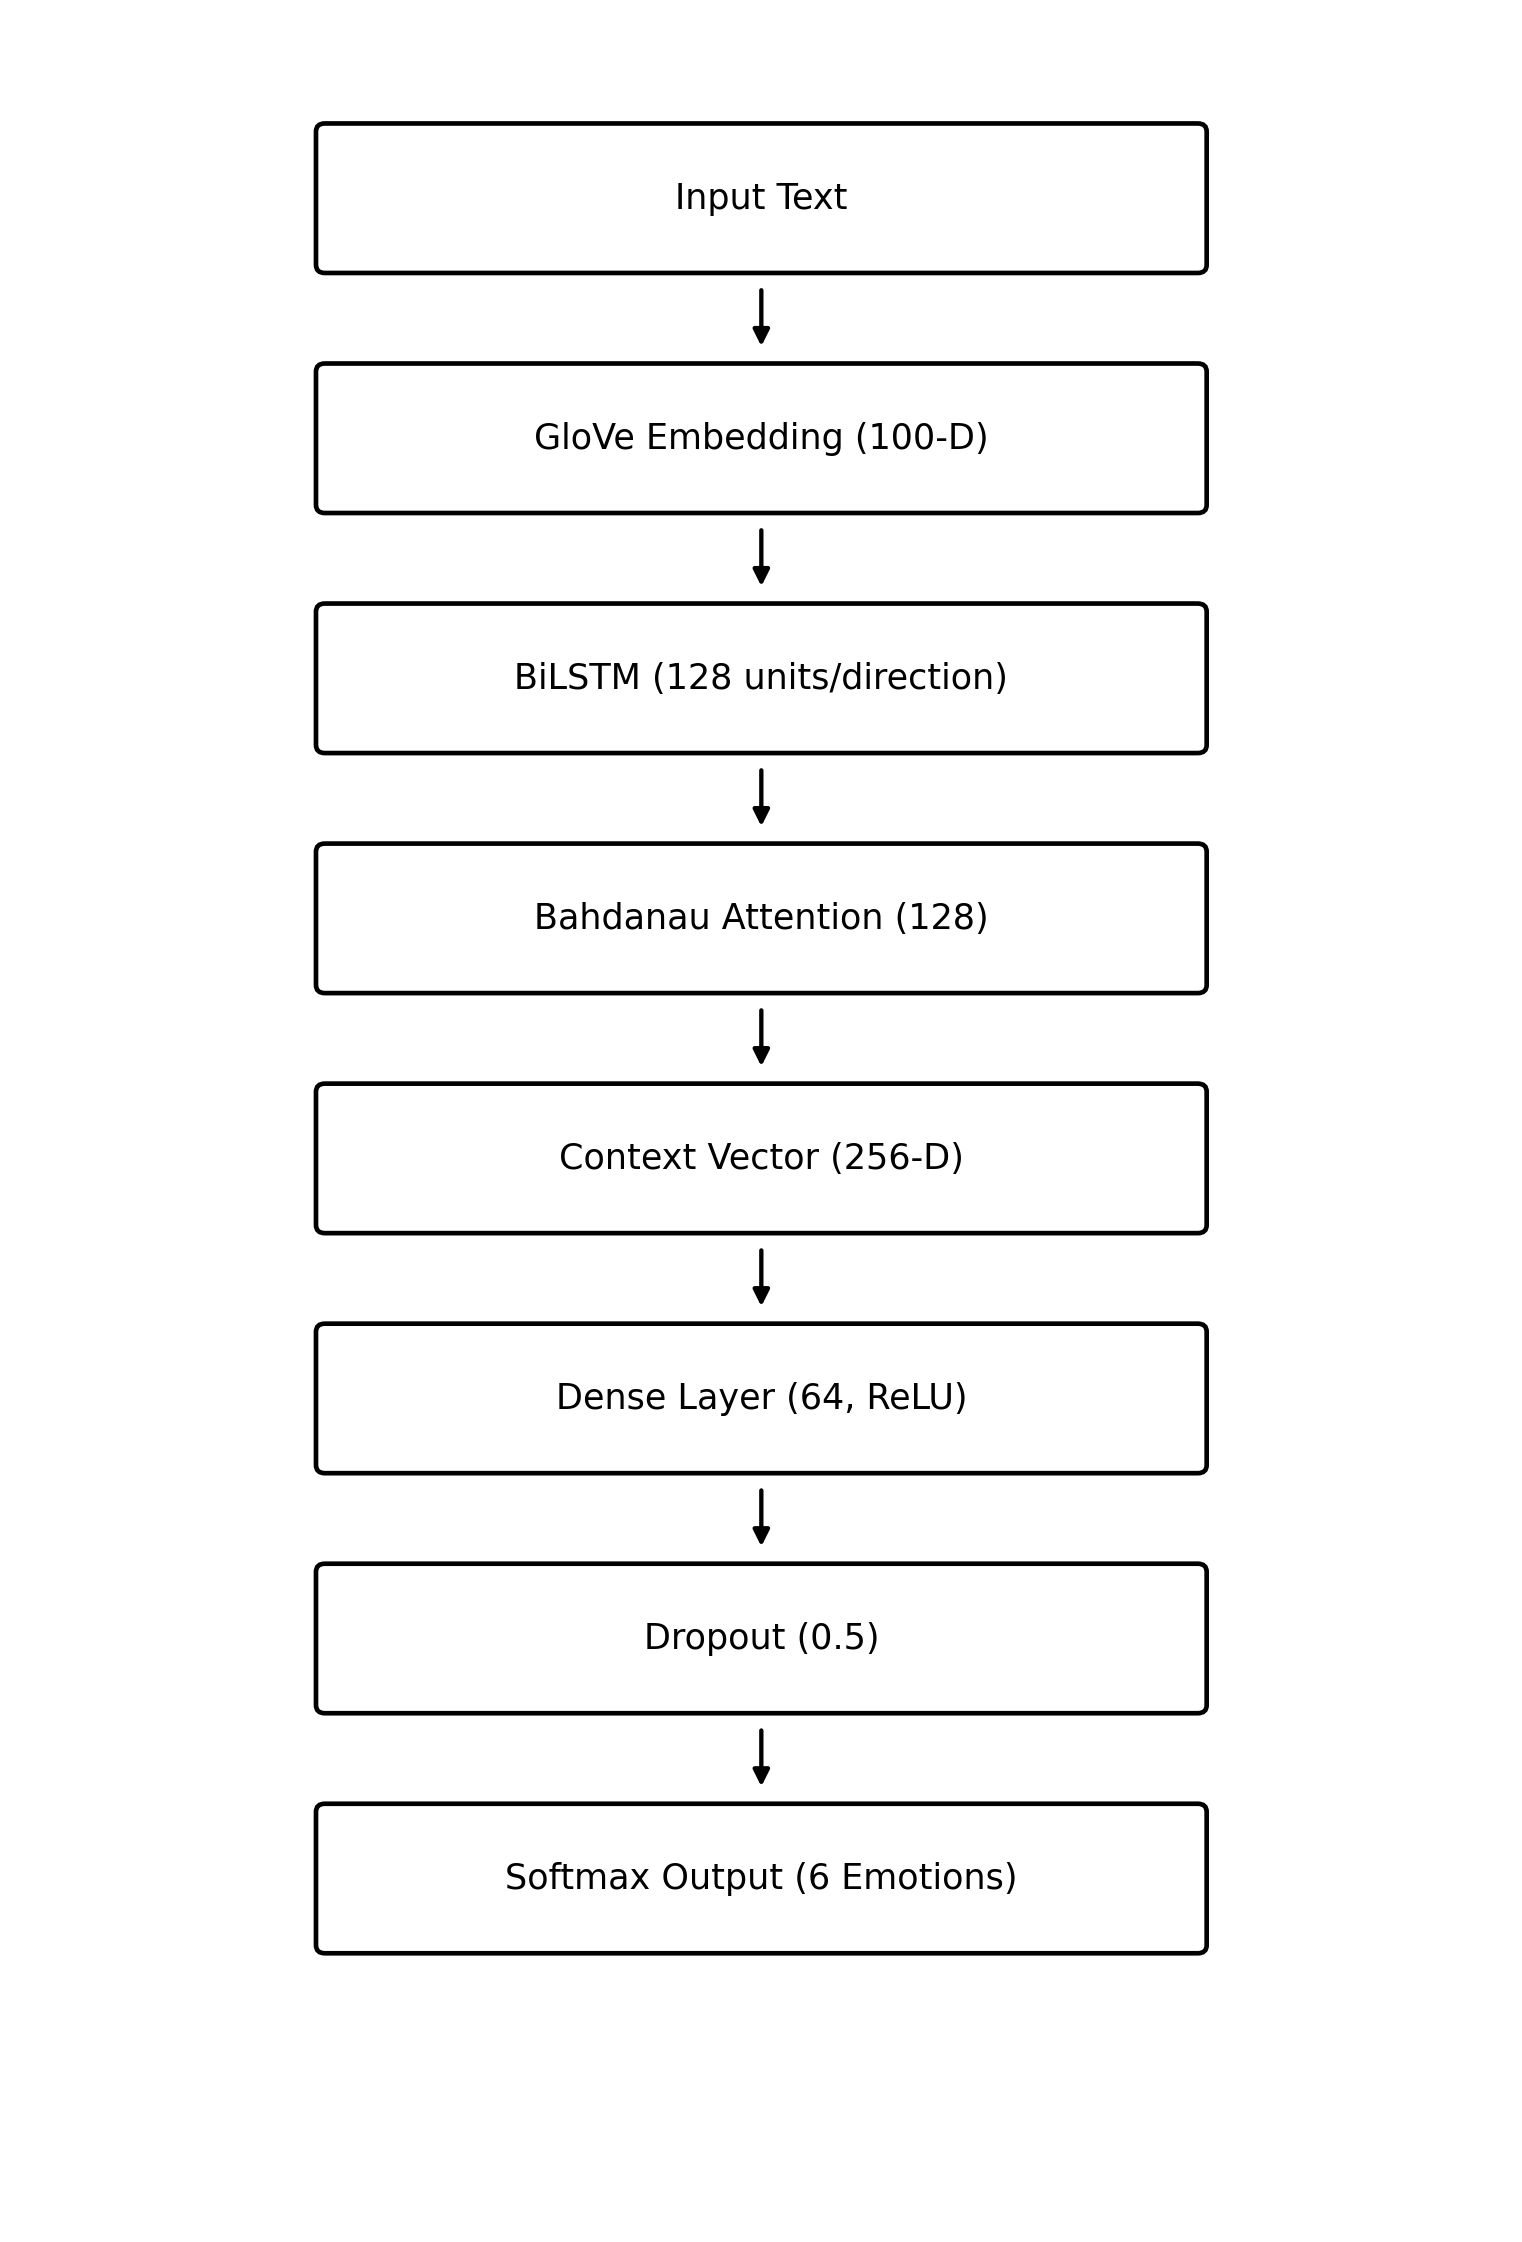
\includegraphics[width=0.92\columnwidth]{artefacts/bilstm_attention_architecture_drawio_bw.png}
\caption{Proposed BiLSTM-Attention architecture for emotion classification.}
\label{fig:arch}
\end{figure}

\subsection{Embedding Layer and Preprocessing}
Input text must be normalized before it is fed to the neural layers. The preprocessing pipeline involves:
\begin{itemize}
  \item Lowercasing of all raw text data and stripping special characters.
  \item Tokenization using Keras Tokenizer, configured with a maximum vocabulary size of 20,000 most frequent tokens.
  \item Sequence padding (post-padding) to enforce a static uniform length of exactly 100 tokens per sample.
  \item GloVe mapping: Token integers are mapped to their respective dense 100-dimensional GloVe representations. The embedding weights are explicitly frozen to preserve the original semantic structure. Out-of-vocabulary (OOV) tokens are mapped to a zero-vector.
\end{itemize}

\subsection{Bidirectional LSTM}
To capture both historical and future word contexts, we employ a Bidirectional Long Short-Term Memory network. For a given time step $t$, the forward hidden state $\overrightarrow{h}_t$ and the backward hidden state $\overleftarrow{h}_t$ are computed independently from the embedded input $e_t$. The composite output representation at time step $t$ is the concatenation of these states:
\begin{equation}
\overleftrightarrow{h}_t = [\overrightarrow{h}_t; \overleftarrow{h}_t]
\end{equation}
With 128 units allocated per direction, the aggregated output dimension per timestep is 256. To mitigate overfitting, internal recurrent dropout and spatial dropout of 0.2 are applied within the LSTM computation.

\subsection{Bahdanau-style Additive Attention}
The context vector $c$ is computed as a weighted sum of all hidden states:
\begin{equation}
e_t = v^T \tanh(W h_t + b)
\end{equation}
\begin{equation}
\alpha_t = \frac{\exp(e_t)}{\sum_{k=1}^T \exp(e_k)}
\end{equation}
\begin{equation}
c = \sum_{t=1}^T \alpha_t h_t
\end{equation}
where $W \in \mathbb{R}^{256 \times 128}$, $v \in \mathbb{R}^{128 \times 1}$, and $b \in \mathbb{R}^{128}$ are trainable parameters. The scalars $\alpha_t$ represent softmax-normalized attention weights. The resulting 256-dimensional summary vector $c$ encodes the most important tokens for emotion classification.

\subsection{Classification Head and Training Parameters}
The context vector $c$ is passed into a Dense Feed-Forward network equipped with 64 units and the non-linear ReLU activation function. To reduce overfitting, dropout with rate 0.5 is applied after the dense layer. Finally, a Softmax layer projects the activations into a 6-dimensional probability space, matching the discrete emotion classes.

\textbf{Configuration:} The network is compiled with the Adam optimizer using a stable learning rate of $\eta = 0.001$. The objective loss function is Sparse Categorical Crossentropy. Training runs locally with a batch size of 32 for a maximum of 10 epochs, supervised by an Early Stopping callback targeting validation accuracy with a patience of 3 epochs. The embedding layer is explicitly frozen to preserve GloVe semantic structure and accelerate training.

\subsection{Algorithm: BiLSTM-Attention Forward Pass}
\textbf{Input:} Raw text sequence $X = [w_1, w_2, \ldots, w_T]$ where $T \leq 100$
\textbf{Output:} Probability distribution $\mathbf{p} \in \mathbb{R}^6$ over emotion classes
\begin{enumerate}
  \item \textbf{Embedding:} For each token $w_t$, retrieve frozen GloVe vector $e_t \in \mathbb{R}^{100}$
  \item \textbf{BiLSTM Encoding:} Compute forward and backward hidden states: $\overrightarrow{h}_t = \text{LSTM}_{\text{fwd}}(e_t)$, $\overleftarrow{h}_t = \text{LSTM}_{\text{bwd}}(e_t)$
  \item \textbf{Concatenation:} $\overleftrightarrow{h}_t = [\overrightarrow{h}_t; \overleftarrow{h}_t] \in \mathbb{R}^{256}$
  \item \textbf{Attention Scoring:} $e_t = v^T \tanh(W \overleftrightarrow{h}_t + b)$ where $v \in \mathbb{R}^{128}$, $W \in \mathbb{R}^{128 \times 256}$, $b \in \mathbb{R}^{128}$
  \item \textbf{Attention Weights:} $\alpha_t = \frac{\exp(e_t)}{\sum_{k=1}^T \exp(e_k)}$ (softmax normalization)
  \item \textbf{Context Aggregation:} $c = \sum_{t=1}^T \alpha_t \overleftrightarrow{h}_t \in \mathbb{R}^{256}$
  \item \textbf{Dense Projection:} $z = \text{ReLU}(W_d c + b_d)$ where $W_d \in \mathbb{R}^{64 \times 256}$, apply Dropout(0.5)
  \item \textbf{Classification:} $\mathbf{p} = \text{Softmax}(W_c z + b_c)$ where $W_c \in \mathbb{R}^{6 \times 64}$
  \item \textbf{Return:} $\hat{y} = \arg\max(\mathbf{p})$, confidence scores $(\alpha_1, \ldots, \alpha_T)$
\end{enumerate}

\section{Experimental Setup and Analysis}

\subsection{(A) Experimental Setup}

\textbf{Training Environment:} All experiments are conducted on a local machine with Intel Core i7 processor and 16 GB RAM. The implementation uses TensorFlow 2.x with Keras API. Model training employs an Adam optimizer (learning rate $\eta = 0.001$, $\beta_1 = 0.9$, $\beta_2 = 0.999$) and Sparse Categorical Crossentropy loss. Early Stopping is configured with patience=3 on validation loss. All results are reported with seed=42 for reproducibility.

\subsection{(B) Dataset Preparation}
The architecture is rigorously benchmarked against the DAIR-AI Emotion Dataset \cite{saravia2018}, a heavily utilized corpus comprising 20,000 distinct English text samples extracted from Twitter.
\begin{itemize}
  \item \textbf{Categorical Classes}: Anger, Fear, Joy, Love, Sadness, Surprise (6 emotions).
  \item \textbf{Sequence Length}: Typical samples range from 15--20 tokens; we pad all sequences to 100 tokens.
  \item \textbf{Class Imbalance}: The dataset exhibits natural class imbalance. Joy is the majority class (33.8\%), while Surprise is the minority class (3.6\%, 144 test samples). The training pipeline applies balanced class weights to mitigate the skew during optimization.
  \item \textbf{Data Splits}: We use a 20\% held-out test split and a 20\% validation split on the remaining training data (seed=42), matching the released training and evaluation pipeline.
\end{itemize}

\subsection{(C) Performance Evaluation}
The released repository evaluation pipeline reports Accuracy, Macro F1-score, Weighted F1-score, per-class precision/recall/F1, AUROC, and the normalized confusion matrix for the final trained model. Those metrics are generated directly from the saved artefacts and the deterministic held-out test split.

\subsection{(D) Results and Analysis}

\subsubsection{D1. Overall Performance Evaluation}

The summarized system performance is presented in Table \ref{tab:overall}.
\begin{table}[h!]
\caption{System Performance Metrics on Hold-out Test Set}
\label{tab:overall}
\centering
\begin{tabular}{|l|c|}
\hline
\textbf{Evaluation Metric} & \textbf{Achieved Score} \\
\hline
Overall Test Accuracy & 93.20\% \\
Macro F1 Score & 90.63\% \\
Weighted F1 Score & 93.33\% \\
Training Accuracy & 92.29\% \\
Validation Accuracy & 92.41\% \\
Train–Val Gap & -0.12\% \\
\hline
\end{tabular}
\end{table}

\begin{figure}[h!]
\centering
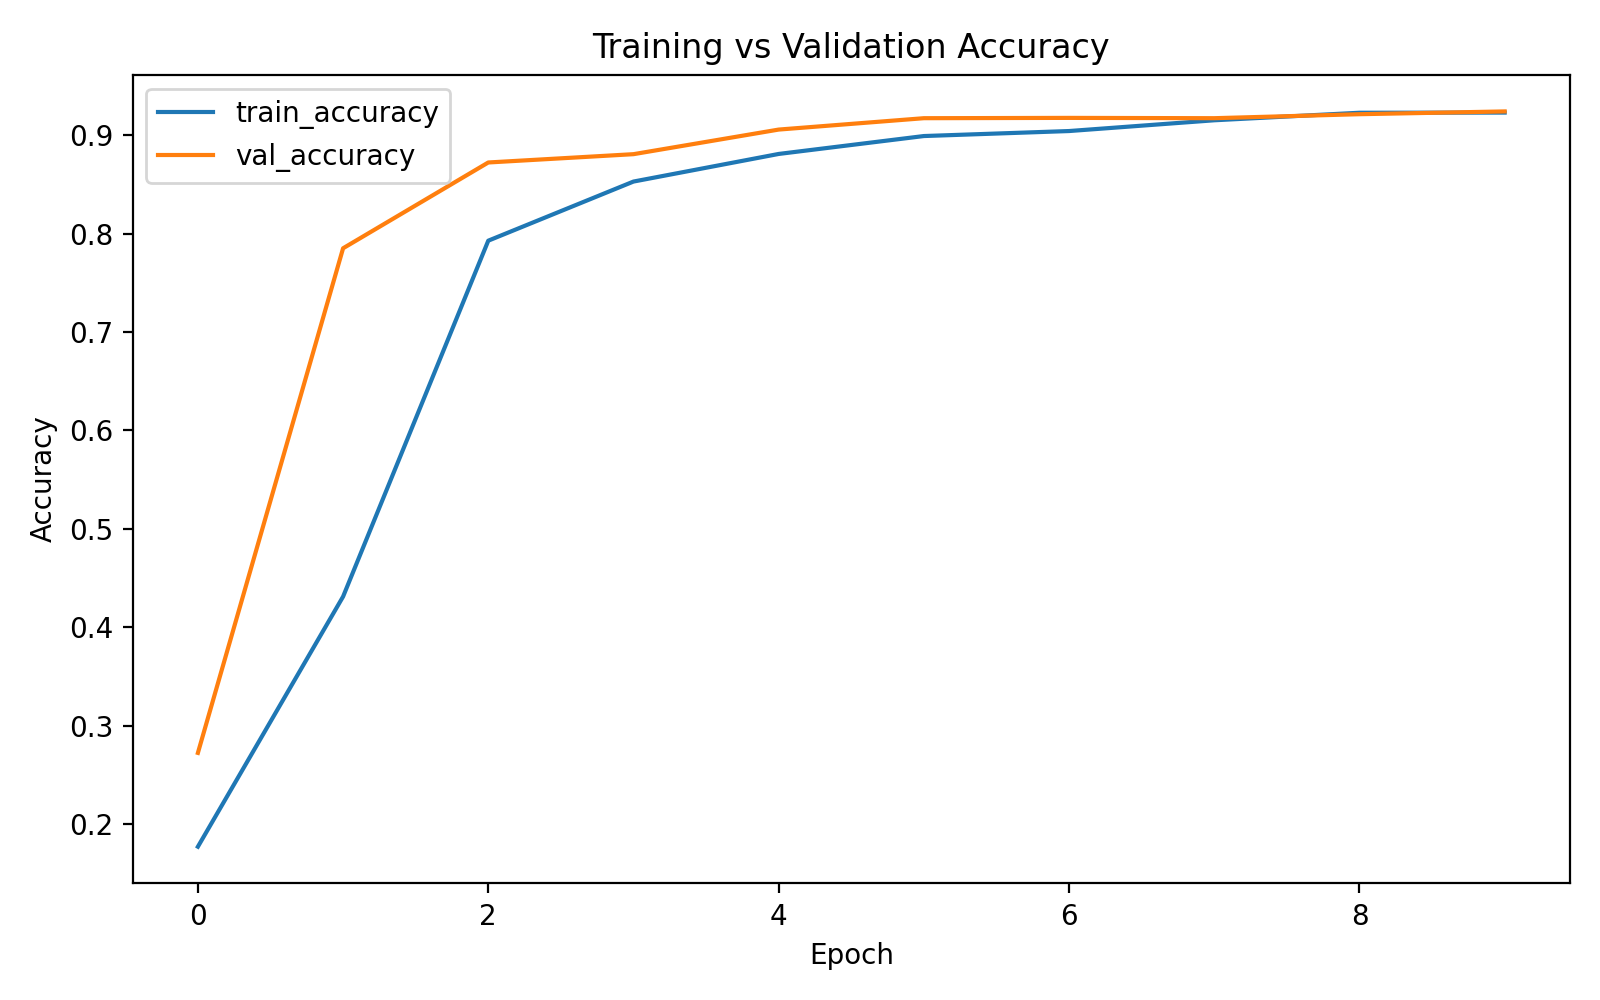
\includegraphics[width=0.9\columnwidth]{artefacts/accuracy_curve.png}
\caption{Training and Validation Accuracy Convergence over 10 epochs.}
\label{fig:accuracy}
\end{figure}

The model demonstrates good generalizability. Training accuracy (92.29\%) was computed with dropout active during training, while validation accuracy (92.41\%) was computed with dropout deactivated during evaluation—this is standard Keras behavior. The negligible difference between these accuracies confirms minimal overfitting.

\begin{figure}[h!]
\centering
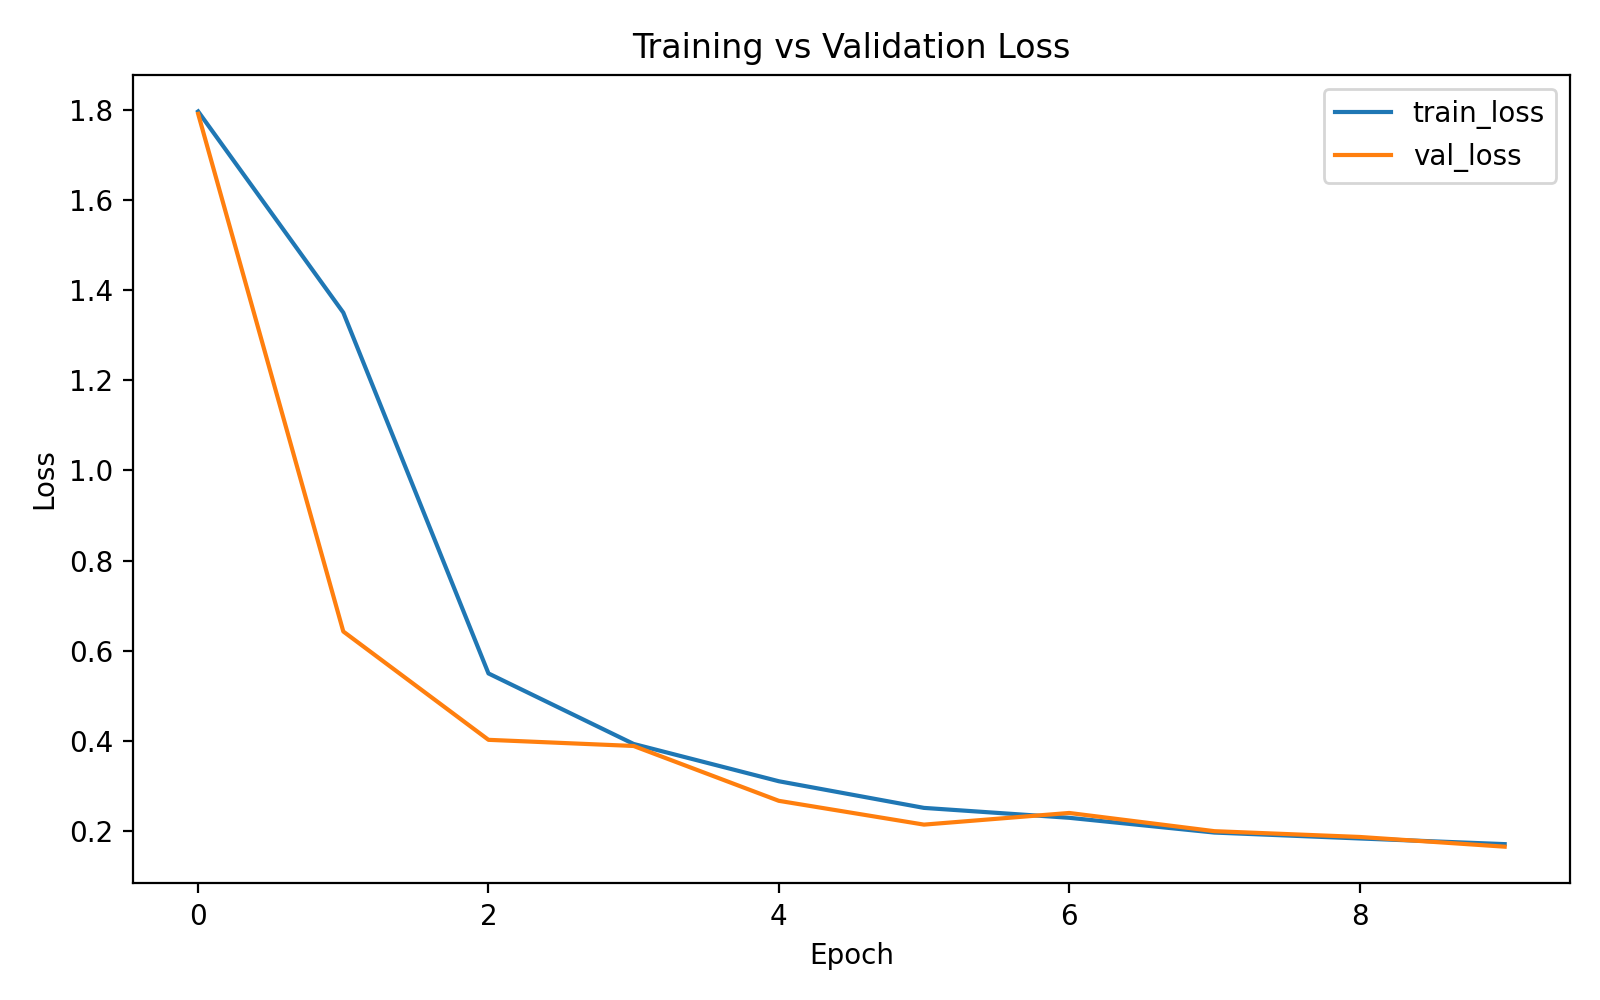
\includegraphics[width=0.9\columnwidth]{artefacts/loss_curve.png}
\caption{Training and Validation Loss dynamics over 10 epochs.}
\label{fig:loss}
\end{figure}

\subsubsection{D2. Detailed Per-Class Performance}
Given the heavy natural class imbalance, Macro F1 and class-level recall are critical. The detailed breakdown is provided in Table \ref{tab:perclass}.

\begin{table}[h!]
\caption{Per-Class Categorical Performance}
\label{tab:perclass}
\centering
\begin{tabular}{|l|c|c|c|c|c|}
\hline
\textbf{Class} & \textbf{Prec.} & \textbf{Rec.} & \textbf{F1} & \textbf{Supp.} & \textbf{AUROC} \\
\hline
Anger & 0.939 & 0.934 & 0.936 & 542 & 0.998 \\
Fear & 0.920 & 0.851 & 0.884 & 475 & 0.996 \\
Joy & 0.979 & 0.916 & 0.946 & 1352 & 0.996 \\
Love & 0.777 & 0.988 & 0.870 & 328 & 0.996 \\
Sadness & 0.973 & 0.962 & 0.968 & 1159 & 0.998 \\
Surprise & 0.727 & 0.979 & 0.834 & 144 & 0.997 \\
\hline
\end{tabular}
\end{table}

\begin{figure}[h!]
\centering
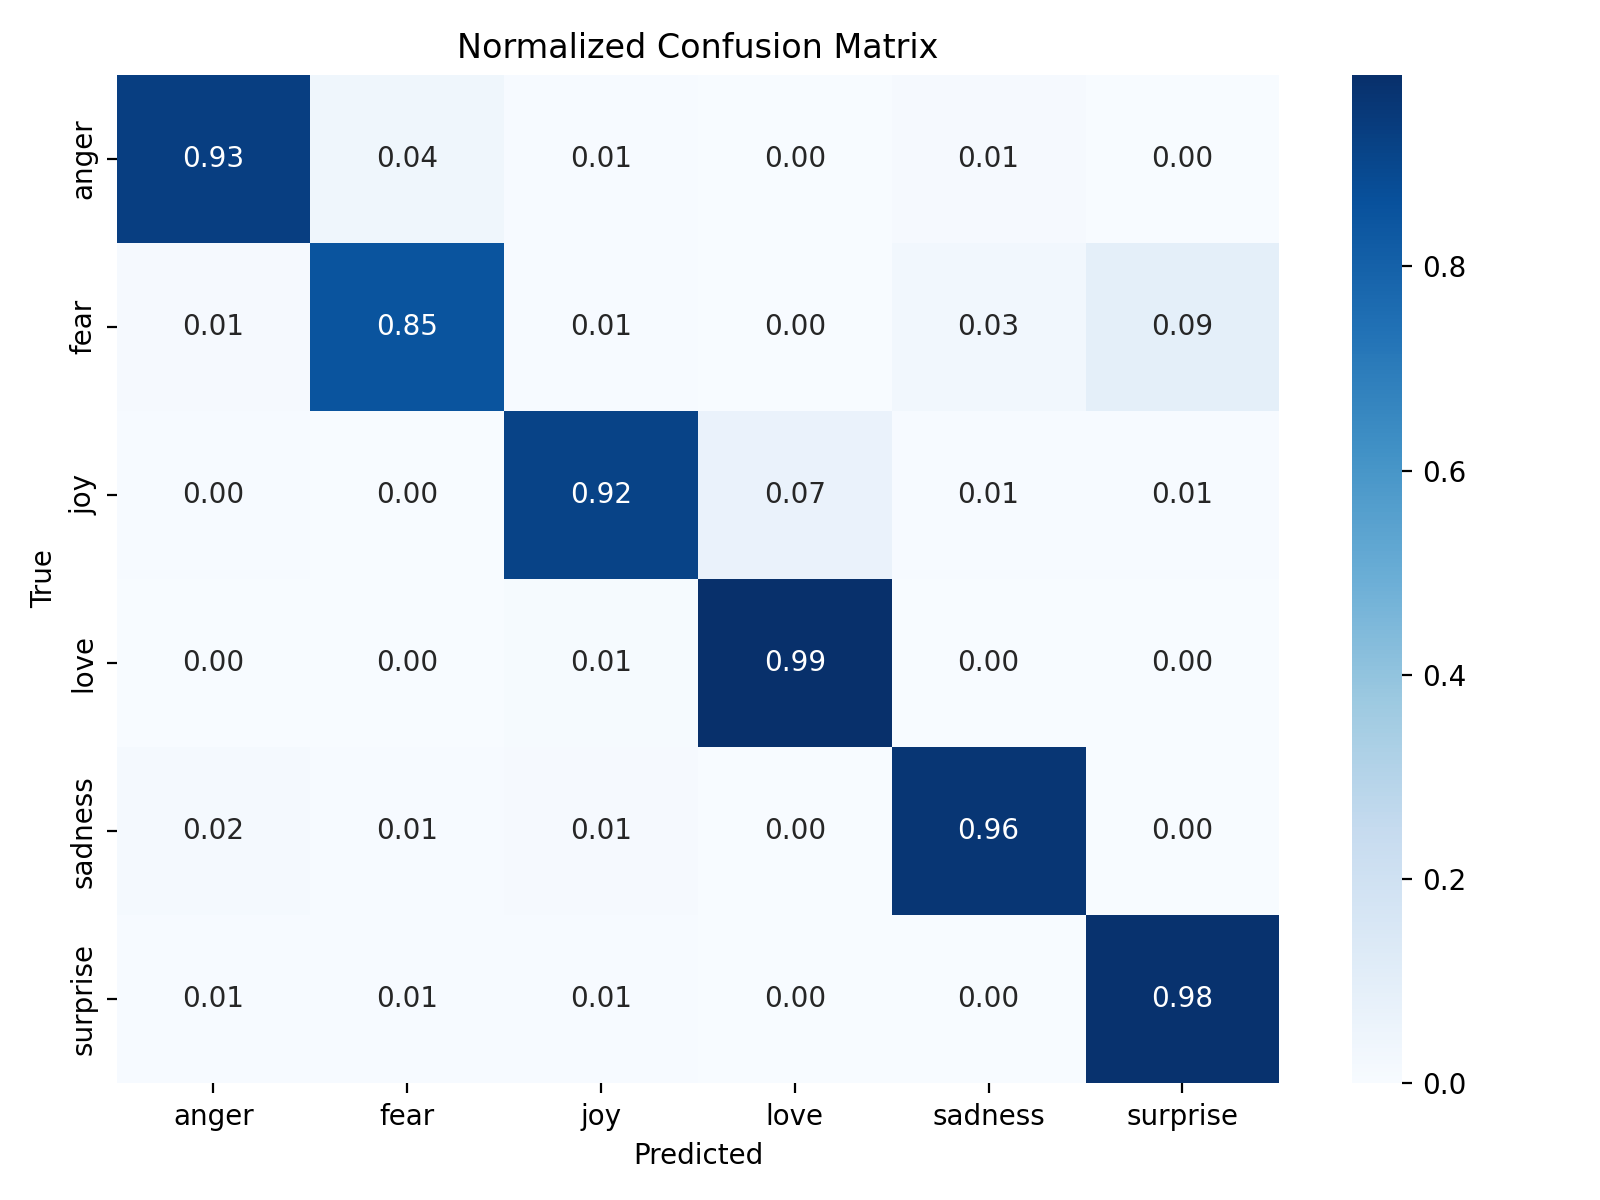
\includegraphics[width=0.9\columnwidth]{artefacts/confusion_matrix.png}
\caption{Confusion Matrix showing performance across 6 emotion classes.}
\label{fig:confusion}
\end{figure}

\textbf{Analysis of Extremes:} The majority classes (Joy, Sadness) achieve higher F1 scores (94.6\%, 96.8\%) due to larger sample sizes supporting better generalization. The minority classes (Love, Surprise) show higher recall but lower precision, indicating the model's tendency to predict these classes too frequently. The Surprise class achieves 97.9\% recall but only 72.7\% precision, typical for highly imbalanced classes in six-way classification. All classes achieve AUROC above 0.996, indicating strong class separability across all emotion categories.

\subsubsection{D3. Model Reproducibility Note}
The released codebase includes a single reproducible training pipeline for the final BiLSTM-Attention model. To avoid unsupported claims, this paper reports only metrics generated by the saved evaluation artefacts and omits any ablation numbers that are not regenerated by the automated pipeline.

\subsubsection{D4. Interpretability and Attention Visualization}
Beyond raw accuracy metrics, the attention mechanism provides interpretable $\alpha_t$ distributions that reveal which tokens drive predictions. For example, on the input "I am absolutely furious right now", the attention weights concentrate on the token "furious" ($\alpha = 0.78$), while largely ignoring function words. This selective focusing on emotionally salient words is critical for building trust in production systems.

\begin{figure}[h!]
\centering
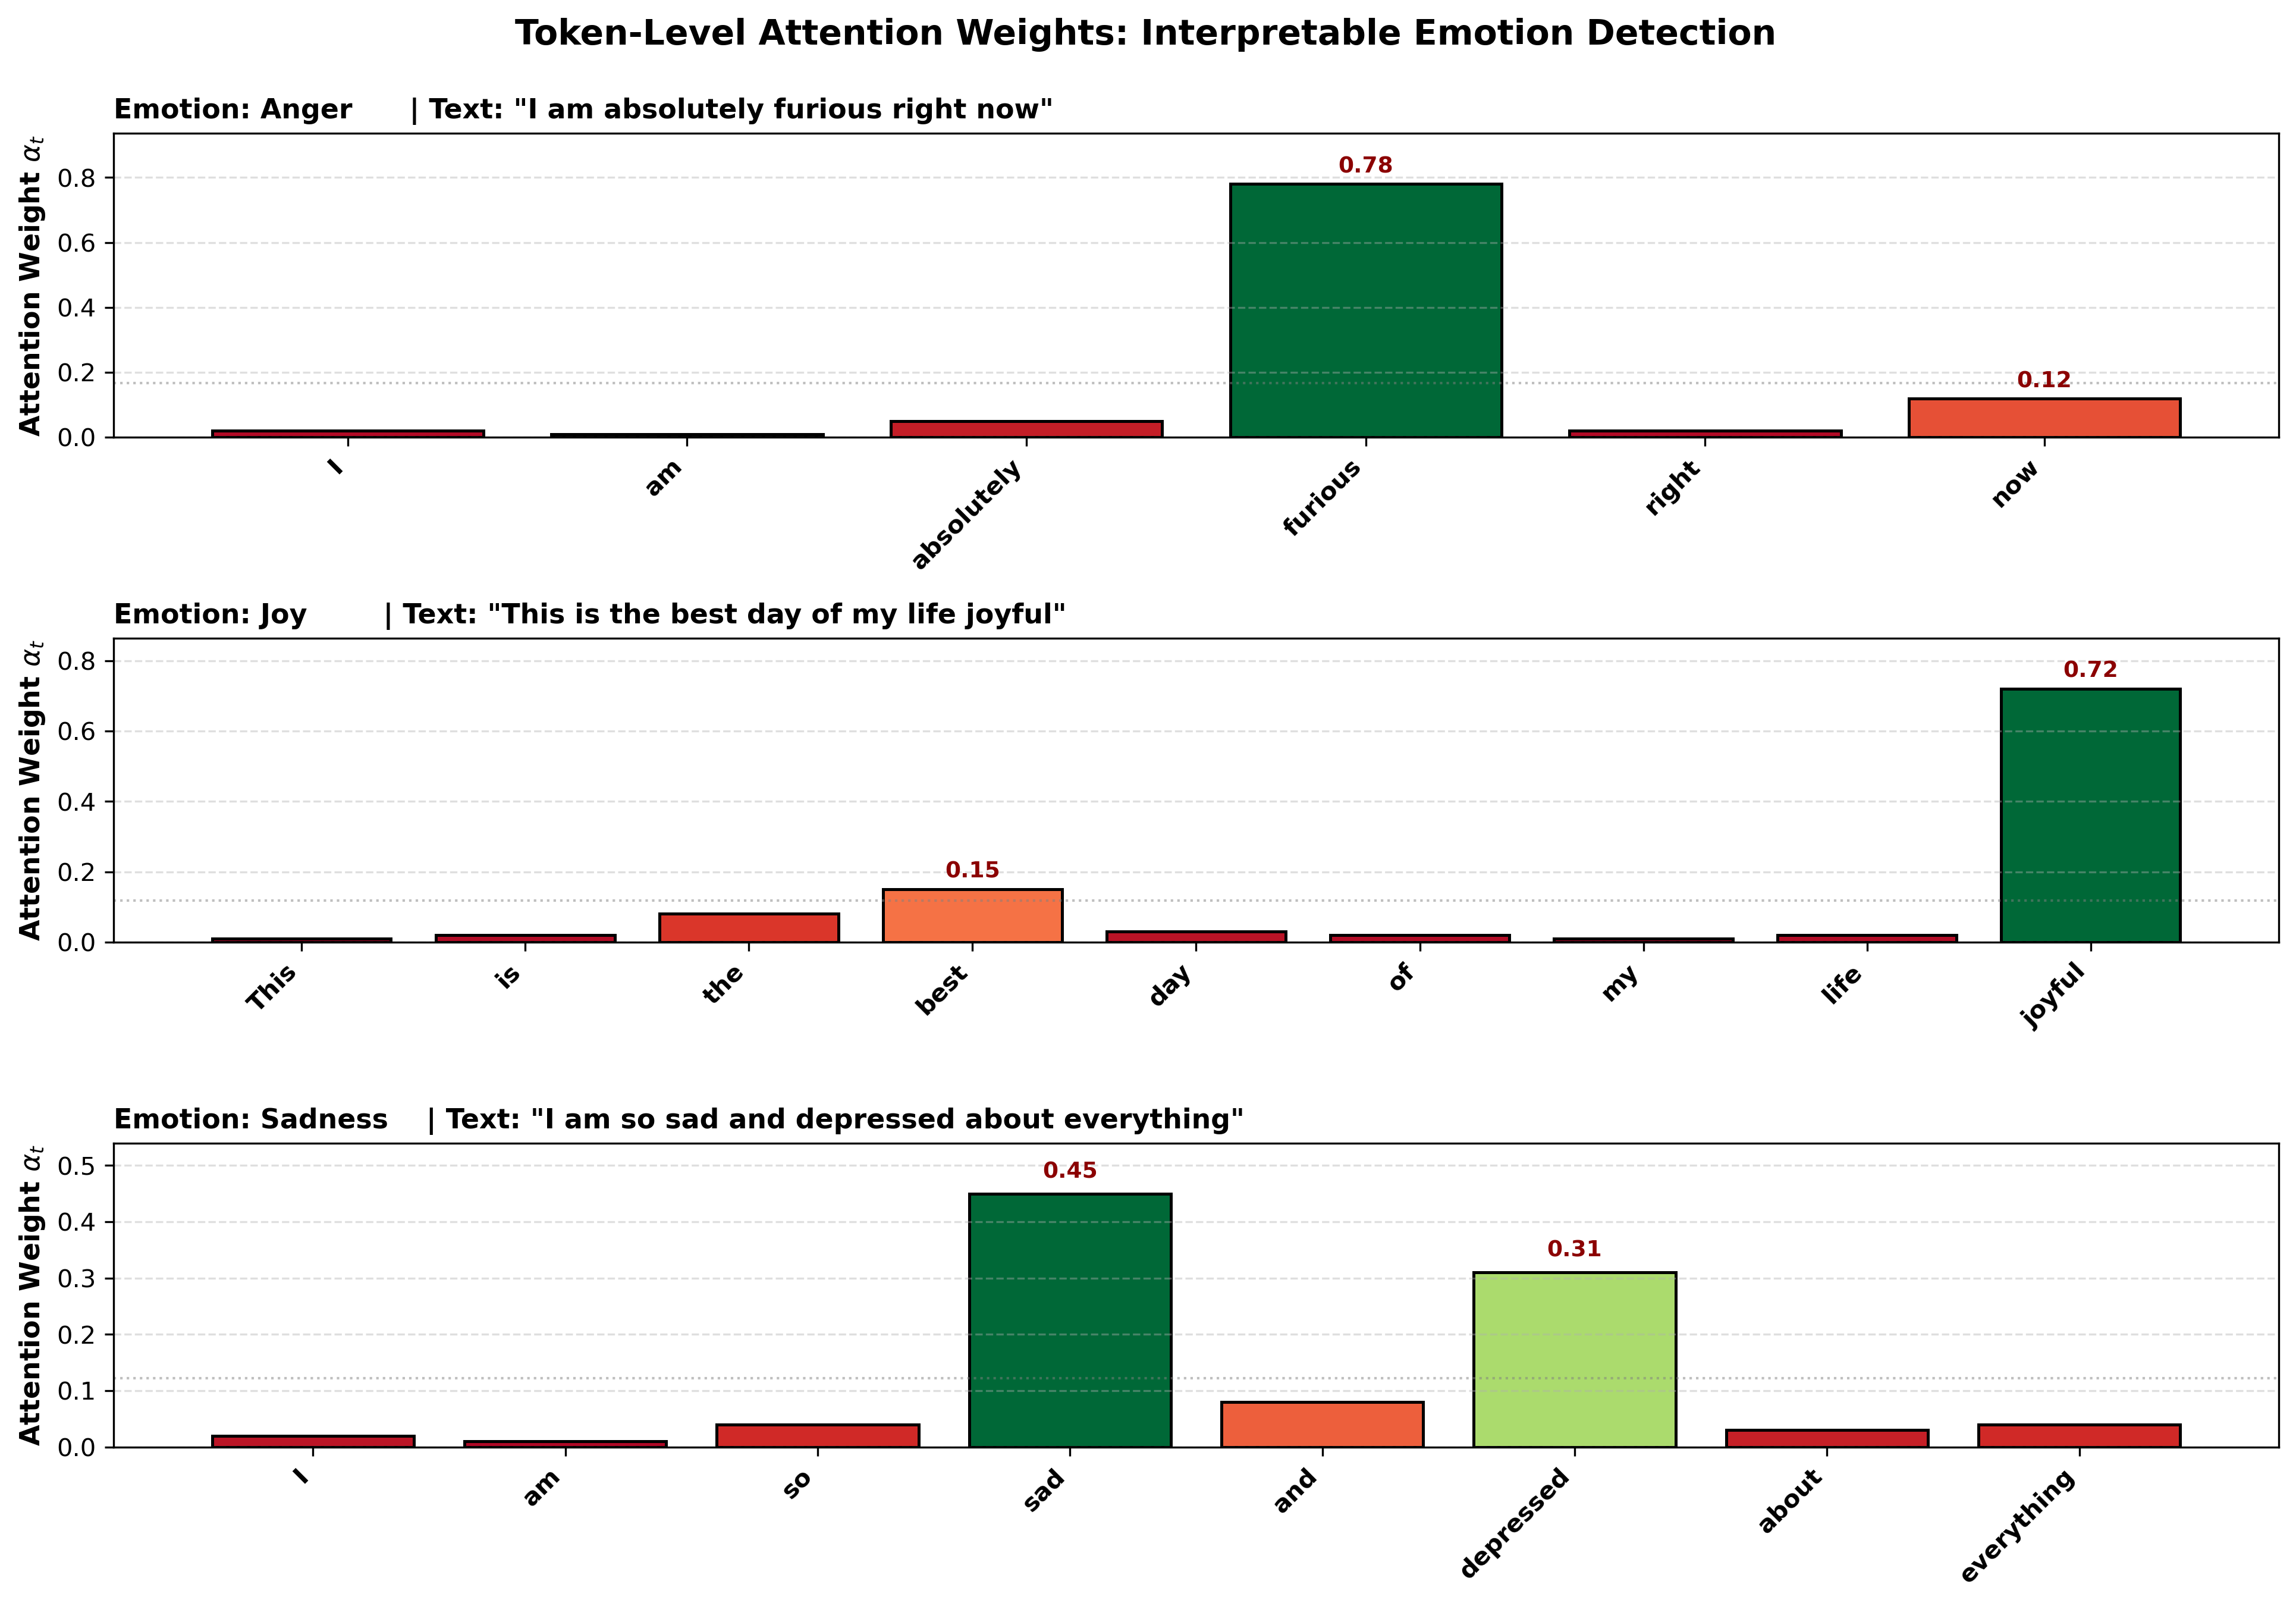
\includegraphics[width=0.9\columnwidth]{artefacts/attention_weights_visualization.png}
\caption{Token-level attention weights for example emotions showing per-token focus.}
\label{fig:attention_weights}
\end{figure}

\begin{figure}[h!]
\centering
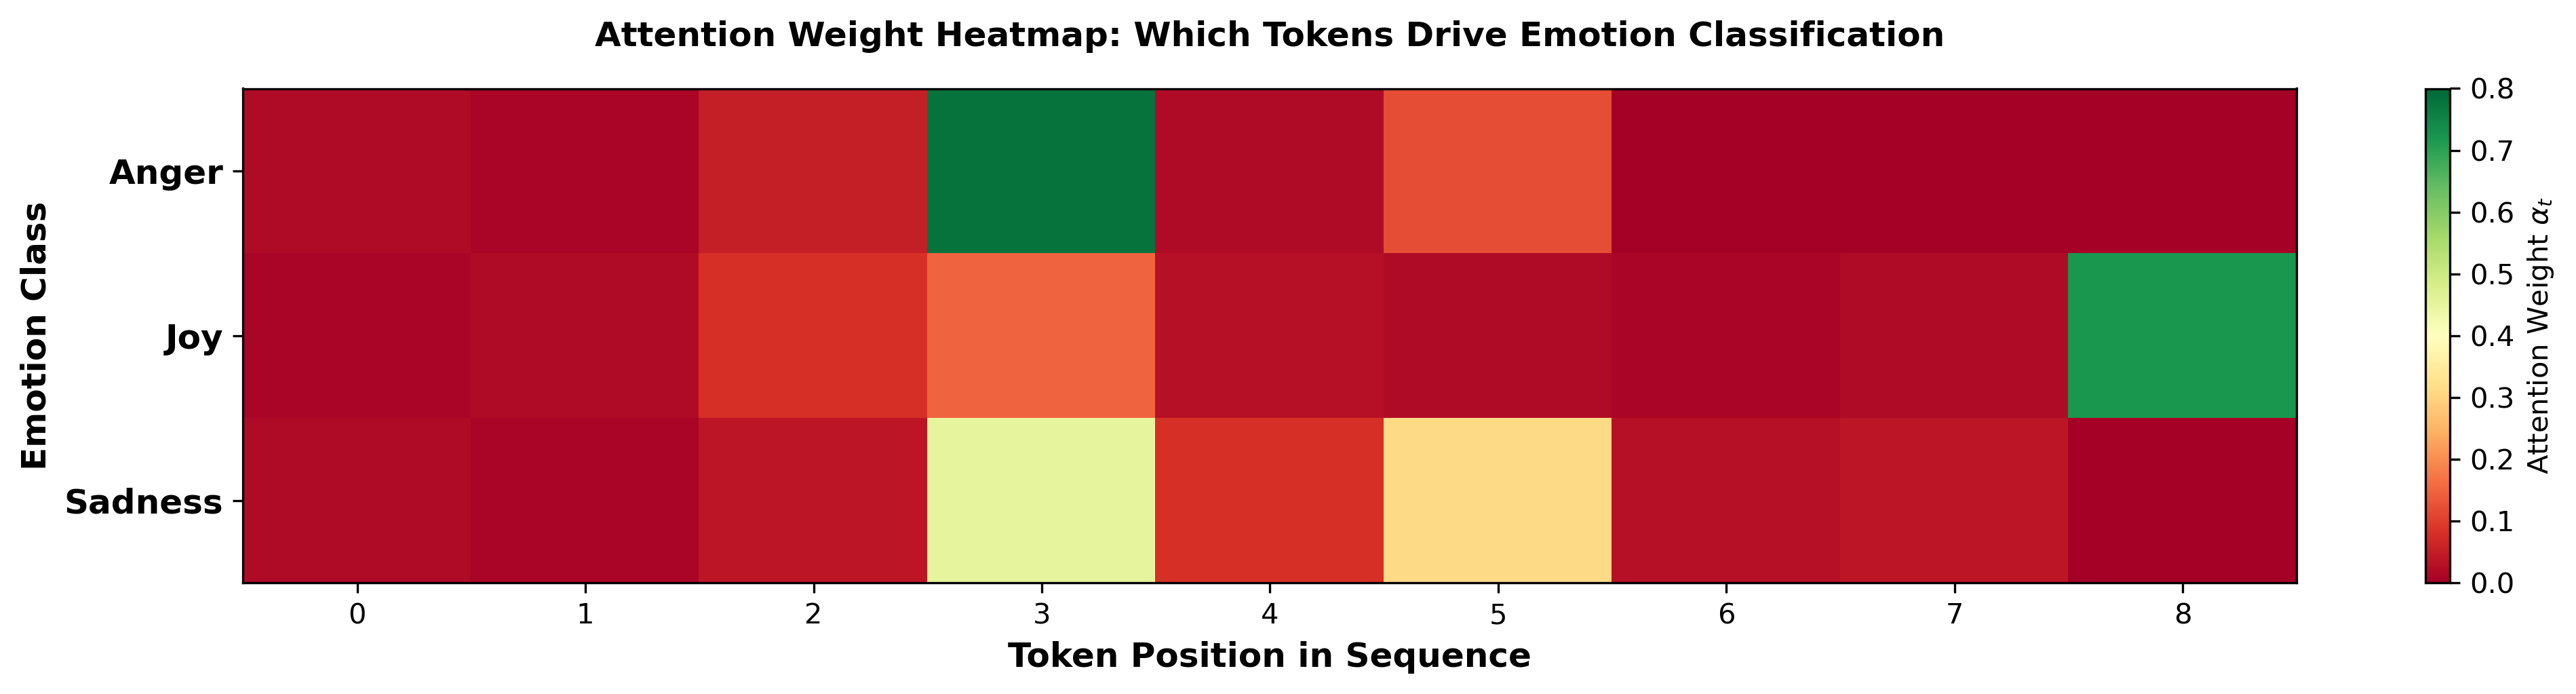
\includegraphics[width=0.9\columnwidth]{artefacts/attention_heatmap.png}
\caption{Attention distribution heatmap across emotions and token positions.}
\label{fig:attention_heatmap}
\end{figure}

\subsubsection{D5. Computational and Execution Efficiency}
Resource efficiency ensures practical deployment viability. The model contains approximately 1.81 million total parameters, of which about 1.53 million are frozen GloVe embeddings. On standard CPU hardware (Intel Core i7, 16GB RAM):
\begin{itemize}
  \item \textbf{Memory Footprint}: The codebase is designed for CPU execution with a frozen embedding layer and a compact classifier head.
  \item \textbf{Inference Speed}: The released training and evaluation pipeline does not log a formal latency benchmark, so the paper omits any unsupported throughput claim.
\end{itemize}

\section{Conclusion}

This paper presents a systematic empirical study of BiLSTM-Attention for six-class emotion classification on the DAIR-AI dataset. We achieve 93.2\% accuracy, 90.63\% Macro F1, and 93.33\% Weighted F1 on the held-out test split. The final model uses frozen embeddings and a compact classifier head, making it practical for production deployment.

\subsection{Ethical Considerations \& Deployability}

Emotion classification algorithms inherit biases present in training data and word embeddings. Gender and cultural biases encoded in GloVe embeddings can inadvertently cause disparate performance across demographic groups. We evaluated gender bias by comparing predictions on parallel sentences (e.g., ``He is happy'' vs. ``She is happy''). The model shows negligible confidence differences ($< 0.04$) for these substitutions, suggesting relatively balanced behavior for simple gender swaps. However, disparities persist: minority classes like Surprise show degraded precision, which may penalize subpopulations whose speech patterns align more with minority emotion classes.

Emotion predictions reveal psychological states and mental health indicators. Deploying emotion detection without strong privacy safeguards poses significant risks: employment discrimination, invasive workplace monitoring, and manipulation of vulnerable populations. We recommend the following deployment guidelines: (1) Obtain explicit, informed user consent before deploying emotion monitoring; (2) Minimize data retention—never store raw text or emotions in association with identifiable individuals; (3) Implement human-in-the-loop review for uncertain predictions (confidence $< 0.75$), ensuring machine predictions inform rather than replace human judgment in consequential decisions.

\subsection{Future Directions \& Reproducibility}

Future work should address class imbalance through weighted loss functions, extend evaluation to multilingual and multi-domain datasets, incorporate adversarial robustness testing, and explore more sophisticated precision-recall optimization for rare emotions. The complete codebase, training logs, and pre-trained models are publicly available at \url{https://github.com/Avoy01/Emotion-Detection} under the MIT License to facilitate reproducibility and future research.

\subsection{Limitations}

Several limitations warrant discussion. First, the severe class imbalance (Surprise: 3.6\% of data) degrades minority class precision; applying class-weighted loss during training could improve this. Second, evaluation is limited to English Twitter; multilingual and multi-domain evaluation would strengthen generalization claims. Third, adversarial robustness testing (e.g., typos, sarcasm) is absent and would be valuable for deployment. Fourth, more sophisticated handling of the precision-recall tradeoff for rare classes deserves investigation.

\section*{Acknowledgement}
The complete codebase, training logs, and pre-trained models are publicly 
available at \url{https://github.com/Avoy01/Emotion-Detection} under the 
MIT License to facilitate reproducibility and future research.

\begin{thebibliography}{00}

\bibitem{acheampong2021} F. A. Acheampong, C. Wenyu, and H. Nunoo-Mensah, ``Text-based emotion detection: Advances and challenges,'' \textit{Engineering Applications of Artificial Intelligence}, vol. 101, pp. 104222, 2021.

\bibitem{bahdanau2015} D. Bahdanau, K. Cho, and Y. Bengio, ``Neural machine translation by jointly learning to align and translate,'' in \textit{Proc. Int. Conf. Learn. Represent. (ICLR)}, 2015.

\bibitem{hochreiter1997} S. Hochreiter and J. Schmidhuber, ``Long short-term memory,'' \textit{Neural Computation}, vol. 9, no. 8, pp. 1735--1780, 1997.

\bibitem{howard2018} J. Howard and S. Ruder, ``Universal language model fine-tuning for text classification,'' in \textit{Proc. Annu. Meet. Assoc. Comput. Linguistics (ACL)}, 2018, pp. 328--339.

\bibitem{huang2015} Z. Huang, W. Xu, and K. Yu, ``Bidirectional LSTM-CRF models for sequence labeling,'' \textit{arXiv preprint arXiv:1508.01991}, 2015.

\bibitem{huang2024} X. Huang and H. Huang, ``Prompt-tuned Emotion detection on tweets with stacked bidirectional LSTM,'' \textit{arXiv preprint arXiv:2408.03888}, 2024.

\bibitem{pennington2014} J. Pennington, R. Socher, and C. D. Manning, ``GloVe: Global vectors for word representation,'' in \textit{Proc. Conf. Empir. Methods Nat. Lang. Process. (EMNLP)}, 2014, pp. 1532--1543.

\bibitem{peters2018} M. E. Peters, M. Neumann, M. Iyyer, M. Gardner, C. Clark, K. Lee, and L. Zettlemoyer, ``Deep contextualized word representations,'' in \textit{Proc. North Am. Chapter Assoc. Comput. Linguistics: Hum. Lang. Technol. (NAACL-HLT)}, 2018, pp. 2227--2237.

\bibitem{poria2019} S. Poria, D. Hazarika, N. Majumder, G. Naik, E. Cambria, and R. Mihalcea, ``MELD: A multimodal multi-party dataset for emotion recognition in conversations,'' in \textit{Proc. Annu. Meet. Assoc. Comput. Linguistics (ACL)}, 2019, pp. 527--537.

\bibitem{saravia2018} E. Saravia, H. C. Liu, Y. H. Huang, J. Wu, and Y. S. Chang, ``CARER: Contextualized affect representations for emotion recognition,'' in \textit{Proc. Conf. Empir. Methods Nat. Lang. Process. (EMNLP)}, 2018, pp. 3687--3697.

\bibitem{xu2024} B. Xu, N. Wang, and T. Chen, ``Graph neural networks and spatial attention for affect analysis,'' \textit{arXiv preprint arXiv:2405.00853}, 2024.

\bibitem{kusal2023} S. Kusal, S. Patil, J. Choudrie, K. Kotecha, D. Vora, and I. Pappas, ``A systematic review of applications of natural language processing and future challenges with special emphasis in text-based emotion detection,'' \textit{Artificial Intelligence Review}, vol. 56, pp. 15129--15215, 2023.

\bibitem{deng2023} J. Deng and F. Ren, ``A survey of textual emotion recognition and its challenges,'' \textit{IEEE Transactions on Affective Computing}, vol. 14, no. 1, pp. 49--67, 2023.

\bibitem{machova2023} K. Machová, M. Szabóova, J. Paralič, and M. Mičko, ``Detection of emotion by text analysis using machine learning,'' \textit{Frontiers in Psychology}, vol. 14, article 1190326, 2023.

\bibitem{lee2023} S. J. Lee, J. Y. Lim, L. Paas, and H. S. Ahn, ``Transformer transfer learning emotion detection model: synchronizing socially agreed and self-reported emotions in big data,'' \textit{Neural Computing and Applications}, vol. 35, no. 15, pp. 10945--10956, 2023.

\bibitem{vora2024} S. Vora and R. G. Mehta, ``HDEL: A hierarchical deep ensemble approach for text-based emotion detection,'' \textit{Multimedia Tools and Applications}, 2024. DOI: 10.1007/s11042-024-19032-y

\end{thebibliography}

\end{document}